\documentclass[11pt,a4paper]{article}

% ---------------------------------------------------------------------------
% Finite-resource amplification can eliminate diagnostic readout windows:
% certified small-threshold instances and large-threshold regimes.
%
% Author metadata: set the macros below before submission.  They are
% deliberately left blank in this version.
% ---------------------------------------------------------------------------
\newcommand{\PaperAuthor}{}
\newcommand{\PaperAffiliation}{}
\newcommand{\PaperDate}{16 September 2026}
\newcommand{\RepositoryNote}{The repository location will be supplied with the author information.}

\usepackage[T1]{fontenc}
\usepackage[utf8]{inputenc}
\usepackage{lmodern}
\usepackage{microtype}
\usepackage[a4paper,margin=1.05in]{geometry}
\usepackage{amsmath,amssymb,amsthm,mathtools}
\usepackage{booktabs}
\usepackage{array}
\usepackage{enumitem}
\usepackage{xcolor}
\usepackage{graphicx}
\usepackage[obeyspaces,spaces]{url}
\usepackage[numbers,sort&compress]{natbib}
\usepackage[colorlinks=true,linkcolor=blue!55!black,citecolor=blue!55!black,urlcolor=blue!55!black]{hyperref}
\hypersetup{pdftitle={Finite-resource amplification can eliminate diagnostic readout windows},
  pdfkeywords={isothermal amplification, detection windows, background amplification, pure-birth process, uniformization, holding times, beta-gamma algebra, formal verification, Lean}}

\DeclareUrlCommand\lean{\urlstyle{tt}}
\setlist{itemsep=2pt,topsep=3pt}
\setlength{\emergencystretch}{1.5em}
\graphicspath{{figures/}}

\theoremstyle{plain}
\newtheorem{theorem}{Theorem}[section]
\newtheorem{proposition}[theorem]{Proposition}
\newtheorem{lemma}[theorem]{Lemma}
\newtheorem{corollary}[theorem]{Corollary}
\theoremstyle{definition}
\newtheorem{definition}[theorem]{Definition}
\theoremstyle{remark}
\newtheorem{remark}[theorem]{Remark}

\newcommand{\R}{\mathbb R}
\newcommand{\N}{\mathbb N}
\newcommand{\Prob}{\mathbb P}
\newcommand{\E}{\mathbb E}
\newcommand{\Var}{\operatorname{Var}}
\newcommand{\Wc}{\mathcal W}
\newcommand{\eps}{\varepsilon}
\newcommand{\dd}{\,\mathrm d}
\newcommand{\one}{\mathbf 1}
\DeclareMathOperator{\Poi}{Poisson}
\DeclareMathOperator{\Gam}{Gamma}
\DeclareMathOperator{\Bet}{Beta}
\DeclareMathOperator{\Ex}{Exp}

% Numbers from large_threshold.py at h = 10^8 (see check_paper.py / BUILD.md).
\newcommand{\tplus}{20.3178}
\newcommand{\tminus}{38.7385}
\newcommand{\muplus}{0.6931}
\newcommand{\muminus}{1.3863}
\newcommand{\BigBlankTwo}{0.009072}
\newcommand{\BigMissTwo}{0.042852}
\newcommand{\BigBlankOne}{0.011712}
\newcommand{\BigMissOne}{0.091891}
\newcommand{\BigTbTwo}{20.4417}
\newcommand{\BigTbOne}{38.4831}
\newcommand{\BigBoundaryTwo}{0.039625}
\newcommand{\BigBoundaryOne}{0.109139}
\newcommand{\BigBoundaryOnePct}{10.914}
\newcommand{\BigBoundaryTwoPct}{3.962}

\title{Finite-resource amplification can eliminate\\ diagnostic readout windows:\\[4pt]
\large certified small-threshold instances and large-threshold regimes}
\author{\PaperAuthor\\ \small \PaperAffiliation}
\date{\PaperDate}

\begin{document}
\maketitle

\begin{abstract}
An amplification reaction may become sensitive enough only after its background-positive probability has already exceeded the permitted limit. We study this timing conflict for an explicit finite-resource birth--immigration source: $z$ active units grow at rate $(b+gz)(1-z/R)$ until an aggregate detection threshold $h$ is reached, a blank starts empty, and a loaded reaction starts with a Poisson number of units. A deadline is acceptable when the blank-positive probability is at most $1\%$ and the missed-call probability at most $5\%$. At threshold five, Poisson mean four, $b=0.01$ and $g=1$ per minute, capacities five, six and seven admit no acceptable deadline at all, capacity eight admits one but none on a $0.1$-minute observation grid, and capacity nine is the least grid-feasible capacity. Capacity ten is feasible at every deadline in $[3.15,3.30]$ minutes, and remains feasible for every fixed rate vector within $2\%$ of nominal, every loading mean at least $3.99$ and every actual deadline in $[3.19,3.21]$ minutes. These statements, including the source law, the monotonicity arguments and the rational exponential enclosures, are verified in Lean~4. A uniform rescaling of all rates cannot create a window; a state-dependent resource change can. We then analyse arbitrarily large thresholds through the independent holding times of the count chain and the beta--gamma algebra. If the capacity exceeds the threshold by a margin that grows without bound, depletion becomes a common additive delay and the undepleted design rules apply after re-centering. If the margin is a fixed number $m$ of units, the last births near exhaustion add an independent $\Gam(m+1)$ delay in logarithmic time, and the limiting error tradeoff depends only on $b/g$, the loading mean and $m$: with these parameters, at most two units of headroom leave no window, three or more do. For every threshold $h\ge10^{8}$ we prove, with explicit constants and without any $h$-state computation, that capacity $h$ has no acceptable deadline while capacity $2h$ has one at an explicit time; the certified instances at threshold five are therefore not an artefact of small counts or of reactions that are positive at time zero. Numerical Laplace inversion at $h=10^{8}$ confirms the bounds. The large-threshold results are conventional proofs and are identified as such. The model is an effective one; no clinical calibration or specific molecular capacity intervention is established.
\end{abstract}

\section{Introduction}\label{sec:intro}

Isothermal nucleic-acid amplification assays such as loop-mediated isothermal amplification (LAMP) \citep{notomi2000} call a reaction positive when an aggregate signal crosses a threshold before a deadline. Two failure modes compete. Stopping too early misses reactions that contain target but have not yet amplified enough; stopping too late lets non-specific background amplification make blank reactions positive \citep{rolando2019,hardinge2019}. In a digital format the target content of a reaction is a Poisson random variable \citep{vogelstein1999}, so both failure probabilities are properties of a stochastic amplification law, and the assay designer needs a deadline at which both are acceptable.

This paper treats that decision for one explicitly defined stochastic source and asks a sharper question than ``which deadline is best'': \emph{does any acceptable deadline exist at all}, and what determines the answer? Let $F_0(t)$ be the probability that a blank has called positive by time $t$ and $M_\lambda(t)$ the probability that a reaction with Poisson mean loading $\lambda$ is still negative at $t$. The acceptable set is
\begin{equation}\label{eq:window}
\Wc_{R,\lambda}=\{t\ge0:\ F_{0,R}(t)\le\alpha,\ M_{R,\lambda}(t)\le\beta\},\qquad \alpha=0.01,\ \beta=0.05,
\end{equation}
where $R$ is the capacity of the source defined in Section~\ref{sec:model}. The distinction between a poorly chosen deadline and an empty $\Wc_{R,\lambda}$ matters in practice: the first is corrected by re-timing, the second only by changing the reaction. A second, more mundane distinction arises when an instrument observes on a fixed time grid: a nonempty continuous window may contain no observation frame.

\paragraph{Context.} The tradeoff itself is established experimental territory. Rolando and colleagues measured amplification efficiency, background and time to threshold across temperatures and polymerases in real-time digital LAMP \citep{rolando2019}, and later combined real-time kinetics with melt curves to separate specific from non-specific products \citep{rolando2020}; the latter observation rule uses information that a timing-only decision does not have. Hardinge and Murray related low-copy quantification to timing and replicate variance \citep{hardinge2020} and reduced false positives with quenched primers \citep{hardinge2019}. Schneider, Blakely and Tripathi modelled product sizes for electrophoretic discrimination \citep{schneider2019}, a different observable. None of these is the subject of the present paper, which is a mathematical case study, and none of the numerical parameters used below is fitted to their data.

\paragraph{Main results in words.} The source is a pure-birth process with immigration and a finite effective resource: from count $z<h$ the next unit appears at rate $(b+gz)(1-z/R)$, and the reaction latches positive at count $h$. With threshold $h=5$, mean loading $\lambda=4$, $b=0.01$ and $g=1$ per minute we prove:
\begin{enumerate}[label=(\roman*)]
\item capacities $R=5,6,7$ admit no acceptable deadline; capacity eight admits one ($3.45$ minutes) but none on the grid $\{0,0.1,0.2,\dots\}$ minutes; capacity nine is grid-feasible at $3.3$ minutes; capacity ten is feasible at every deadline in $[3.15,3.30]$ minutes (Theorem~\ref{thm:capacity});
\item capacity ten remains feasible for every fixed state-specific rate vector within $2\%$ of nominal, every loading mean at least $3.99$ and every actual deadline in $[3.19,3.21]$ minutes (Theorem~\ref{thm:robust});
\item multiplying all rates by a common factor rescales the window and cannot create one (Proposition~\ref{prop:clock}); a fixed-rate-constant mass-action realization of the source inherits the continuous capacity classification but not the grid classification (Proposition~\ref{prop:massaction}).
\end{enumerate}
Items (i)--(iii) are checked in Lean~4 with Mathlib \citep{demoura2021,mathlib2020}, from the probability law down to the rational enclosures of the exponentials involved. They concern a six-state chain, and a legitimate objection is that a real detector fires at counts many orders of magnitude larger, where $37\%$ of loaded reactions are not already positive at time zero as they are here. Section~\ref{sec:large} answers this with conventional proofs:
\begin{enumerate}[label=(\roman*),resume]
\item the threshold time is a sum of independent exponential holding times whose undepleted part has an exact beta law; with a growing capacity margin $R-h\to\infty$, depletion is asymptotically a deterministic additive delay and the limiting tradeoff is the undepleted one (Theorem~\ref{thm:reserve}); with a fixed margin $R=h+m$, the last births contribute an independent $\Gam(m+1)$ delay in logarithmic time (Theorem~\ref{thm:headroom}), and the limiting tradeoff is a function of $(b/g,\lambda,m)$ alone;
\item for every integer $h\ge10^{8}$, capacity $R=h$ has no acceptable deadline and capacity $R=2h$ has one at an explicit time, with explicit error bounds (Theorem~\ref{thm:big}). The proof uses four scalar enclosures and no computation of dimension $h$.
\end{enumerate}
Numerical Laplace-transform inversion, which also costs $O(h)$ rather than $O(h^2)$, corroborates the bounds at $h=10^{8}$ and shows the finite-threshold tradeoffs converging to their limits.

\paragraph{Three kinds of evidence.} Every statement below carries one of three labels. \emph{Lean-verified} statements are theorems in the frozen Lean~4/Mathlib development described in Section~\ref{sec:verification}; they depend only on the standard axioms. \emph{Conventional} statements are proved in the text with ordinary mathematics; their scalar enclosures are replayed with directed rounding by the script \path{check_paper.py}. \emph{Numerical} statements are floating-point evaluations, labelled as such, and are never premises of a theorem. Section~\ref{sec:verification} lists which results fall in which class.

\paragraph{What is not claimed.} The units of the source are effective amplification units, not nucleotides or fluorescence; the rate constants are illustrative; the capacity is an effective inventory whose laboratory realization is an open question discussed in Section~\ref{sec:mechanism}; the public data replay in Section~\ref{sec:data} validates a crossing rule, not the model. Neither clinical performance nor priority over the experimental literature is asserted.

\paragraph{Organization.} Section~\ref{sec:model} defines the source, the probability law and the deadline sets. Section~\ref{sec:certified} states the certified threshold-five theorems. Section~\ref{sec:mechanism} analyses the mechanism, clock changes, loading and a mass-action realization. Section~\ref{sec:large} contains the large-threshold theory. Section~\ref{sec:data} discusses data, a discriminating experiment and sampling confidence. Section~\ref{sec:verification} describes verification and reproducibility, and Section~\ref{sec:conclusion} concludes. Appendices~\ref{app:exact}--\ref{app:map} contain the exact source calculation, the comparison lemmas, the proof of Theorem~\ref{thm:big}, the directed arithmetic and the claims-to-declarations map.

\section{The effective finite-resource source}\label{sec:model}

\subsection{Counts, capacity and latch}\label{sec:source}
Fix an integer threshold $h\ge1$, an integer capacity $R\ge h$, a background coefficient $b>0$ and a growth coefficient $g>0$. Let $z\in\{0,\dots,h\}$ be the number of active signal units; $R-z$ is the remaining effective precursor inventory. Before detection the only transition is $z\mapsto z+1$, at rate
\begin{equation}\label{eq:rates}
q_R(z)=(b+gz)\Bigl(1-\frac zR\Bigr),\qquad 0\le z<h.
\end{equation}
The detector latches positive when the count reaches $h$, and the reaction is then stopped: state $h$ is absorbing. The factor $b$ is background initiation, $gz$ is growth proportional to the active count, and $1-z/R$ is the resource factor. Both target-origin and background-origin units grow with the same coefficient, so their sum is a closed observable and no independence of resource-sharing lineages is assumed. There is no activation delay, extinction, optical error or between-run heterogeneity. Except where stated, $h=5$, $b=1/100$ and $g=1$ per minute; time is in minutes.

A \emph{blank} starts at $z=0$. A \emph{loaded} reaction has $N\sim\Poi(\lambda)$ potential active units and initially activates $\min(N,R)$ of them, consuming inventory; its stopped initial state is $\min(N,h)$. A load at or above threshold is positive at time zero; this is part of the source and is neither discarded nor renormalized.

\subsection{The probability law used in the proofs}\label{sec:law}
The formal development defines all probabilities through uniformization \citep{jensen1953,grassmann1977}, avoiding any unverified simulation. For the six-state instances $5\le R\le10$ take the common rate $\nu=5/2$ per minute, which bounds every $q_R(z)$ (the largest is $q_{10}(4)=2.406$). The kernel $P_R$ on $\{0,\dots,5\}$ is
\begin{equation}\label{eq:kernel}
P_R(z,z+1)=q_R(z)/\nu,\qquad P_R(z,z)=1-q_R(z)/\nu\quad(z<5),\qquad P_R(5,5)=1,
\end{equation}
with all other entries zero; every entry is nonnegative and each row sums to one. Let $f(z)=\one_{\{z<5\}}$ be the uncalled indicator. The survival (uncalled) probability from state $z$ at time $t$ is the Poisson mixture
\begin{equation}\label{eq:source}
S_R(t,z)=\sum_{n=0}^{\infty}e^{-\nu t}\frac{(\nu t)^n}{n!}\,(P_R^nf)(z),
\end{equation}
which is the transition law of the continuous-time chain with rates \eqref{eq:rates} \citep{norris1997}. The operating probabilities are
\begin{align}
F_{0,R}(t)&=1-S_R(t,0),\label{eq:blank}\\
M_{R,\lambda}(t)&=\sum_{n=0}^{\infty}e^{-\lambda}\frac{\lambda^n}{n!}\,S_R\bigl(t,\min(n,5)\bigr)
=e^{-\lambda}\sum_{n=0}^{4}\frac{\lambda^n}{n!}\,S_R(t,n).\label{eq:miss}
\end{align}
The second equality is exact: loads $n\ge5$ are absorbed at time zero and contribute no negative calls. All probabilities and error limits are per reaction.

Since the count never decreases, a positive latch at deadline $t$ is equivalent to threshold attainment by $t$. On the observation grid $G=\{k/10:k\in\N\}$ minutes, anchored at zero, the acceptable frames are $\Wc_{R,\lambda}\cap G$. All statements use a fixed threshold and deterministic deadlines.

\subsection{Monotonicity and the separating-time principle}\label{sec:monotone}
The survival $S_R(t,z)$ is nonincreasing in $t$ (Appendix~\ref{app:exact}, Lemma~\ref{lem:antitone}), hence $F_{0,R}$ is nondecreasing and $M_{R,\lambda}$ nonincreasing. Two consequences organise every negative and every positive result below.

\begin{lemma}[Separating time]\label{lem:separating}
If some $s\ge0$ satisfies $F_{0,R}(s)>\alpha$ and $M_{R,\lambda}(s)>\beta$, then $\Wc_{R,\lambda}=\varnothing$.
\end{lemma}
\begin{proof}
If $t\le s$ then $M_{R,\lambda}(t)\ge M_{R,\lambda}(s)>\beta$; if $t\ge s$ then $F_{0,R}(t)\ge F_{0,R}(s)>\alpha$. Every $t\ge0$ falls in one of the two cases.
\end{proof}

\begin{lemma}[Interval structure]\label{lem:interval}
$\Wc_{R,\lambda}$ is an interval, closed in $[0,\infty)$. If $s\le u$ are feasible then every $t\in[s,u]$ is feasible.
\end{lemma}
\begin{proof}
For $s\le t\le u$, $F_{0,R}(t)\le F_{0,R}(u)\le\alpha$ and $M_{R,\lambda}(t)\le M_{R,\lambda}(s)\le\beta$. Closedness follows from the continuity of the finite spectral expression \eqref{eq:spectral}.
\end{proof}
Thus an empty window is certified by one separating time, and a whole interval of feasible deadlines by its two endpoints. No interpolation between sampled times is involved.

\section{Certified results at threshold five}\label{sec:certified}

\subsection{Minimum capacity and observation grid}
\begin{theorem}[Minimum capacity and timing allowance; Lean-verified]\label{thm:capacity}
For the source \eqref{eq:rates}--\eqref{eq:miss} with $h=5$ and $\lambda=4$:
\begin{enumerate}[label=(\alph*)]
\item $\Wc_{5,4}=\Wc_{6,4}=\Wc_{7,4}=\varnothing$, while $3.45\in\Wc_{8,4}$;
\item $\Wc_{8,4}\cap G=\varnothing$, while $3.3\in\Wc_{9,4}\cap G$;
\item $[3.15,3.30]\subseteq\Wc_{10,4}$.
\end{enumerate}
Consequently the least feasible integer capacity among $R\ge5$ is eight with continuous deadlines and nine on the prescribed grid.
\end{theorem}

\begin{proof}
Appendix~\ref{app:exact} derives the exact finite spectral form of \eqref{eq:source} and certifies the inequalities in the last column of Table~\ref{tab:certs} by rational enclosures. For capacities five, six and seven the listed time is a separating time, so Lemma~\ref{lem:separating} applies. For capacity eight the evaluation at $3.45$ meets both limits. Every grid point is either at most $3.4$ or at least $3.5$: the miss bound at $3.4$ and monotonicity exclude the first set, the blank bound at $3.5$ the second. The capacity-nine witness $3.3$ lies on the grid. These statements exhaust the admissible smaller capacities; no monotonicity of feasibility in $R$ is used. For (c), Lemma~\ref{lem:interval} with the two endpoint bounds for capacity ten.
\end{proof}

\begin{table}[htbp]\centering\small
\begin{tabular}{rrrrl}\toprule
$R$ & $t$ (min) & $F_{0,R}(t)$ & $M_{R,4}(t)$ & Certified inequality\\\midrule
5 & 5.00 & $.01355402$ & $.06920700$ & both $>\alpha,\beta$ (separating)\\
6 & 4.00 & $.01076152$ & $.05773912$ & both $>\alpha,\beta$ (separating)\\
7 & 3.67 & $.01026447$ & $.05146115$ & both $>\alpha,\beta$ (separating)\\
8 & 3.45 & $.00976997$ & $.04923440$ & both $\le\alpha,\beta$ (witness)\\
8 & 3.40 & --- & $.05070654$ & miss $>\beta$ (excludes frames $\le3.4$)\\
8 & 3.50 & $.01012746$ & --- & blank $>\alpha$ (excludes frames $\ge3.5$)\\
9 & 3.30 & $.00940708$ & $.04807559$ & both $\le\alpha,\beta$ (grid witness)\\
10 & 3.15 & --- & $.04857072$ & miss $\le\beta$ (interval endpoint)\\
10 & 3.30 & $.00991967$ & --- & blank $\le\alpha$ (interval endpoint)\\\bottomrule
\end{tabular}
\caption{Source evaluations behind Theorem~\ref{thm:capacity}. The decimals are numerical displays of the exact spectral formula; Lean verifies the inequalities in the last column through rational enclosures (Appendix~\ref{app:exact}).}
\label{tab:certs}
\end{table}

\begin{figure}[htbp]\centering
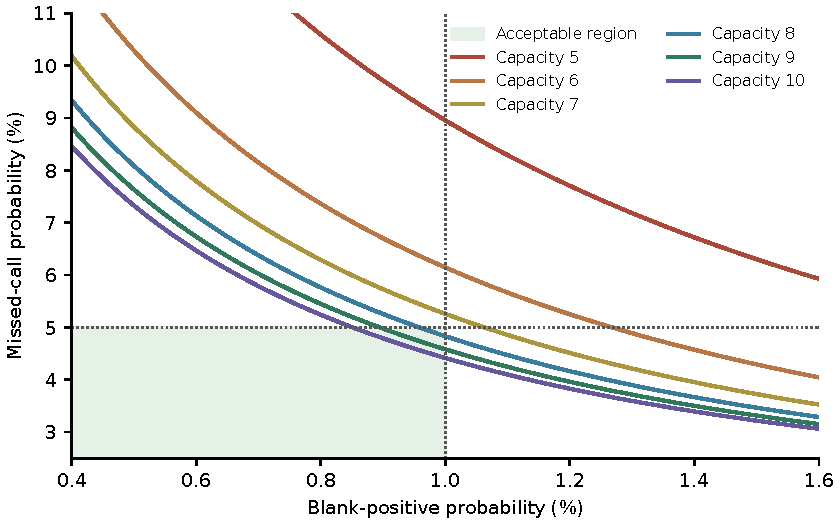
\includegraphics[width=.9\linewidth]{tradeoff.pdf}
\caption{The error tradeoff as the deadline varies, for capacities five to ten; the lower-left rectangle is acceptable. Additional capacity advances both desired and background amplification. Curves are numerical evaluations of the exact spectral formula; the theorem rests on the certified points of Table~\ref{tab:certs}, not on plotted intersections.}\label{fig:tradeoff}
\end{figure}

Numerically, the full windows are about $[3.4237,3.4822]$ minutes for capacity eight (about $3.5$ seconds wide), $[3.2346,3.3824]$ for capacity nine and $[3.1029,3.3110]$ for capacity ten (Figure~\ref{fig:frames}); capacities six and seven have their sensitivity endpoint after their blank endpoint ($4.268>3.889$ and $3.721>3.632$). These root locations are not formal claims. The grid statement in (b) concerns the grid anchored at zero; a phase-shifted six-second grid could intersect the capacity-eight window, so the observation schedule is part of the decision problem.

\begin{figure}[htbp]\centering
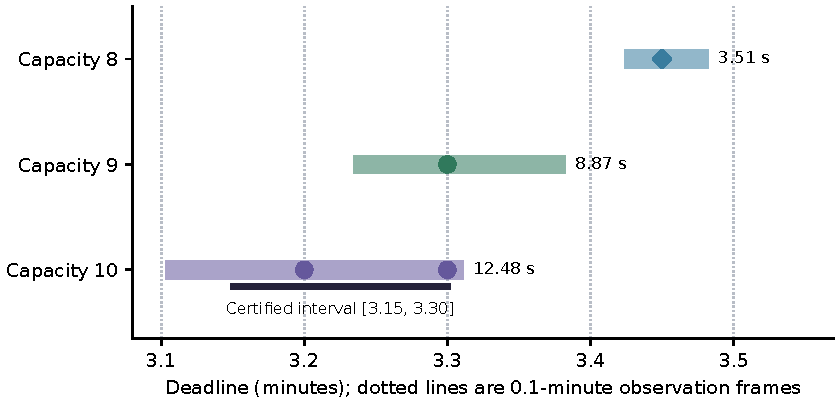
\includegraphics[width=.9\linewidth]{observation_windows.pdf}
\caption{Magnified deadline windows. Bars use numerical endpoints; circles mark feasible six-second frames; the diamond is the certified continuous capacity-eight witness and the black segment the certified capacity-ten interval. Capacity eight has a window but no frame on this grid.}\label{fig:frames}
\end{figure}

\subsection{A uniform operating tolerance}
The same source permits a guarantee over a continuum of fixed rate vectors, loading means and actual observation times; it is not a statement about time-varying or random rate fluctuations within a reaction.

\begin{theorem}[Rate, loading and timing tolerance; Lean-verified]\label{thm:robust}
Let $q_z=q_{10}(z)$ be the nominal capacity-ten rates. For every fixed vector with $0.98\,q_z\le\widetilde q_z\le1.02\,q_z$ for $0\le z<5$, every loading mean $\lambda\ge3.99$ and every actual deadline $t\in[3.19,3.21]$ minutes, the source with rates $\widetilde q$ satisfies $F_{0,\widetilde q}(t)\le0.01$ and $M_{\widetilde q,\lambda}(t)\le0.05$.
\end{theorem}

\begin{proof}
Appendix~\ref{app:comparisons} proves, for the law \eqref{eq:source}, that increasing state-specific rates advances threshold crossing (Lemma~\ref{lem:rateorder}), that increasing the loading mean reduces missed calls (Lemma~\ref{lem:loadorder}), and that scaling every rate by $c$ replaces $t$ by $ct$ (Lemma~\ref{lem:scaling}). The largest allowed rate, $1.02\times2.406$, is below $\nu=5/2$, so all comparisons live under the common uniformization clock. Hence
\begin{align*}
F_{0,\widetilde q}(t)&\le F_{0,1.02q}(t)=F_{0,q}(1.02t)\le F_{0,q}(3.2742)\le.01,\\
M_{\widetilde q,\lambda}(t)&\le M_{0.98q,3.99}(t)=M_{q,3.99}(0.98t)\le M_{q,3.99}(3.1262)\le.05,
\end{align*}
where the last two inequalities are rationally certified evaluations of the exact source (numerically $.00973128$ and $.04967252$).
\end{proof}
The theorem allows $2\%$ variation in each pre-threshold rate and $\pm0.6$ seconds around a nominal $3.2$-minute deadline (Figure~\ref{fig:robust}). It does not assert that a laboratory assay meets these tolerances or that rate uncertainty is its only uncertainty. The two worst cases need not occur under one rate vector; each bounds its own error for every admitted vector, which is what a joint operating requirement needs.

\begin{figure}[htbp]\centering
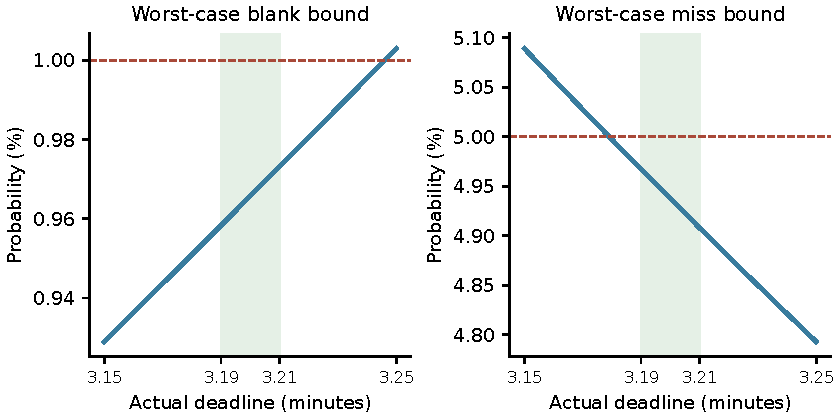
\includegraphics[width=.9\linewidth]{uncertainty.pdf}
\caption{Worst-case comparison bounds for capacity ten: the blank curve uses rates $1.02q$, the miss curve $0.98q$ with loading $3.99$. Shading marks the certified actual-time interval; dashed lines are the error limits. Curves are numerical; the guarantee follows from the comparison lemmas and the two certified endpoint bounds.}\label{fig:robust}
\end{figure}

\section{Mechanism, clocks, loading and a mass-action realization}\label{sec:mechanism}

\subsection{Why capacity changes feasibility and a common clock cannot}
The resource factor in \eqref{eq:rates} depends on the current count. A blank traverses the whole chain from zero; a loaded reaction starts at a random higher count and traverses a shorter final segment. Changing $R$ changes the state-dependent delays of these two populations differently and thereby the error tradeoff. By contrast:

\begin{proposition}[Common clock invariance; Lean-verified]\label{prop:clock}
If every rate is multiplied by $c>0$, then $F_0^{(c)}(t)=F_0(ct)$, $M_\lambda^{(c)}(t)=M_\lambda(ct)$ and $\Wc^{(c)}=c^{-1}\Wc$. In particular a continuous window exists for the scaled source if and only if it exists for the original.
\end{proposition}
\begin{proof}
Lemma~\ref{lem:scaling}; the bijection $t\mapsto ct$ preserves existence.
\end{proof}
Common acceleration can move which grid frames a window contains but cannot create a window. With depletion removed altogether (rates $b+gz$), the otherwise identical mean-four source has numerical blank and miss probabilities $.00949563$ and $.03721034$ at $2.8$ minutes, an acceptable deadline; the capacity-five source has miss $.20452023$ at that time and, by Theorem~\ref{thm:capacity}, no acceptable deadline anywhere. An undepleted approximation therefore predicts a usable deadline where the finite-resource source has none. The undepleted comparison is numerical; the all-deadline exclusion is certified.

\subsection{Loading requirements}
For each fixed deadline, $M_{R,\lambda}(t)$ is nonincreasing in $\lambda$ (Lemma~\ref{lem:loadorder}). Empty-loaded reactions follow the blank law, so retaining the $N=0$ term of \eqref{eq:miss} gives, whenever the blank constraint holds,
\begin{equation}\label{eq:floor}
M_{R,\lambda}(t)\ \ge\ e^{-\lambda}S_R(t,0)\ \ge\ e^{-\lambda}(1-\alpha).
\end{equation}
Feasibility therefore requires $\lambda\ge\log\bigl((1-\alpha)/\beta\bigr)=\log(0.99/0.05)\approx2.98568$. At $\lambda=4$ the floor is about $0.0181$, well below $\beta$; capacity five fails for kinetic reasons, not for lack of loading. Defining $\lambda_{\min}(R)=\inf\{\lambda:\Wc_{R,\lambda}\ne\varnothing\}$, the boundary is located numerically where the miss at the latest blank-admissible time equals $\beta$:
\[
\begin{array}{c|cccccc}
R&5&6&7&8&9&10\\\hline
\lambda_{\min}(R)&4.9490&4.2892&4.0666&3.9562&3.8899&3.8456
\end{array}
\]
At the fixed capacity-ten deadline $3.2$ the threshold is about $3.9253$. These are not clinical limits of detection: relating specimen concentration to activated units needs an extraction, capture and activation model.

\subsection{What the capacity comparison holds fixed, and a mass-action realization}\label{sec:massaction}
The capacity comparison in Theorem~\ref{thm:capacity} holds $\lambda$, $b$ and the undepleted growth coefficient $g$ fixed. It does not assert that adding reagent to a fixed-volume assay realises that comparison. Consider the elementary reactions $P\to X$ and $P+X\to2X$ at fixed volume $V$ with rate constants $k_b$ and $k_g$, where $R$ is the conserved total $P+X$. Their propensity at $X=z$ is
\begin{equation}\label{eq:massaction}
q^{\mathrm{MA}}_R(z)=k_b(R-z)+\frac{k_g}{V}\,z(R-z)=\kappa R\,(a+z)\Bigl(1-\frac zR\Bigr),\qquad \kappa=\frac{k_g}{V},\quad a=\frac{k_b}{\kappa}.
\end{equation}
Matching \eqref{eq:rates} with $g=1$ requires $b=a$, and the physical rates are the normalized rates multiplied by $\kappa R$. Two consequences follow.

\begin{proposition}[Fixed-rate-constant family; conventional]\label{prop:massaction}
For the family \eqref{eq:massaction} with $a=1/100$, $\Wc^{\mathrm{MA}}_{R,\lambda}=(\kappa R)^{-1}\Wc_{R,\lambda}$. Hence at $\lambda=4$ and threshold five, capacities five, six and seven admit no deadline and eight is the least feasible capacity, exactly as in Theorem~\ref{thm:capacity}, with no change of $k_b$ or $k_g$. The grid classification does not transfer: with $\kappa=0.1$ and $k_b=0.001$ (so that capacity ten has the nominal clock), capacity eight's window becomes $[4.2796,4.3528]$ minutes, which contains the frame $4.3$ (numerically blank $.00969904$, miss $.04952343$), so eight is grid-feasible in this family.
\end{proposition}
\begin{proof}
Proposition~\ref{prop:clock} with $c=\kappa R$ applied capacity by capacity; the numerical window follows from Table~\ref{tab:certs}'s method at normalized time $3.44$.
\end{proof}
In this family a pre-threshold initial count $n$ means $X(0)=n$ and $P(0)=R-n$; a protocol that adds $n$ targets to a fixed inventory $R$ has total $R+n$ and is a different loaded source, a distinction that matters when $n/R$ is appreciable. Other suggested mechanisms (Michaelis--Menten substrate dependence, reporter saturation, finite surface occupancy, droplet-volume variation) change the source in different ways: a reporter ceiling alone changes the observation map, not the birth rates, and a saturating factor $(R-z)/(K+R-z)$ with substrate far above $K$ has little rate effect. They must be modelled separately rather than relabelled to preserve the present law.

\subsection{Initial detection and the case for large thresholds}\label{sec:initial}
At threshold five and mean four, $\Prob(N\ge5)\approx0.371163$: about $37\%$ of loaded reactions are positive at time zero. This is part of the stated source and limits a literal interpretation in which a handful of captured molecules must amplify substantially before detection. Depletion is also substantial near detection: at $z=4$ the resource multiplier is $0.2$ for capacity five and $0.6$ for capacity ten. The next section shows that neither feature is responsible for the phenomenon: at $h=10^{8}$ the initially positive fraction is below $10^{-10^{7}}$, and the contrast between $R=h$ and $R=2h$ persists with explicit constants.

\section{Large thresholds: holding times and two regimes}\label{sec:large}

Throughout this section $g=1$ (dimensionless time $gt$), $a=b/g>0$, and $h\to\infty$. Everything is conventional mathematics; Section~\ref{sec:verification} lists the formal obligations that a Lean development of this section would have to discharge.

\subsection{Holding-time representation}
Let $T_{R,h,n}$ be the threshold time of the chain with rates \eqref{eq:rates} started at $n<h$.

\begin{lemma}[Holding times; conventional]\label{lem:holding}
Let $E_n,E_{n+1},\dots,E_{h-1}$ be independent unit exponential variables. Then
\begin{equation}\label{eq:holding}
T_{R,h,n}\ \overset{d}{=}\ \sum_{z=n}^{h-1}\frac{E_z}{q_R(z)}
=\frac{R}{R+a}\Bigl[\sum_{z=n}^{h-1}\frac{E_z}{z+a}+\sum_{z=n}^{h-1}\frac{E_z}{R-z}\Bigr].
\end{equation}
\end{lemma}
\begin{proof}
A pure-birth chain holds in state $z$ for an $\Ex(q_R(z))$ time and moves to $z+1$; successive holding times are independent by the strong Markov property \citep{feller1968,norris1997}. Equivalently, thinning the common Poisson clock of \eqref{eq:source} at state $z$ with probability $q_R(z)/\nu$ produces the same law. The identity $\frac{R}{(z+a)(R-z)}=\frac{R}{R+a}\bigl[\frac1{z+a}+\frac1{R-z}\bigr]$ is partial fractions.
\end{proof}
This replaces any $h$-state matrix by a sum of independent terms. The first sum in \eqref{eq:holding} is the undepleted threshold time; the second is the resource delay. They share the same $E_z$ and are not independent at finite $h$.

\subsection{The startup law}
\begin{lemma}[Beta law of the undepleted time; conventional]\label{lem:beta}
Let $A_{h,n}=\sum_{z=n}^{h-1}E_z/(z+a)$. Then $e^{-A_{h,n}}\sim\Bet(n+a,\,h-n)$ and, with $W_n\sim\Gam(n+a,1)$,
\begin{equation}\label{eq:startup}
A_{h,n}-\log h\ \Rightarrow\ -\log W_n\qquad(h\to\infty).
\end{equation}
Moreover there exist, on an extension of the probability space, $Z\sim\Gam(h+a,1)$ and $W_n\sim\Gam(n+a,1)$ with $A_{h,n}=\log Z-\log W_n$ exactly.
\end{lemma}
\begin{proof}
For $s\ge0$, $\E e^{-sA_{h,n}}=\prod_{z=n}^{h-1}\frac{z+a}{z+a+s}=\frac{\Gamma(n+a+s)\,\Gamma(h+a)}{\Gamma(n+a)\,\Gamma(h+a+s)}$, which is the $s$th moment of $\Bet(n+a,h-n)$; the moments determine a law on $[0,1]$. For the coupling, draw $Z\sim\Gam(h+a,1)$ independent of $e^{-A_{h,n}}$ and set $W_n=Ze^{-A_{h,n}}$; by the beta--gamma algebra \citep{lukacs1955} the product of independent $\Gam(h+a)$ and $\Bet(n+a,h-n)$ variables is $\Gam(n+a)$. Since $Z/(h+a)\to1$ in probability, \eqref{eq:startup} follows. (The variables $Z$ and $W_n$ are not independent; nothing below uses independence between them.)
\end{proof}
The law \eqref{eq:startup} is the classical logarithmic limit of the Yule process with immigration \citep{kendall1948}: a reaction that starts with $n$ units behaves, after $\log h$ units of dimensionless time, like a $\Gam(n+a)$ ``effective initial mass''. Its $n=0$ member, $\Gam(a)$ with $a=0.01$, is extremely spread; this spread is the whole difficulty of separating blanks from loaded reactions by timing.

\subsection{Growing reserve: depletion becomes a common delay}
Write $T=A+D$ with $D_{R,h,n}=T_{R,h,n}-A_{h,n}=\sum_{z=n}^{h-1}\frac{zE_z}{(z+a)(R-z)}$ under the coupling of Lemma~\ref{lem:holding}.

\begin{theorem}[Reserve regime; conventional]\label{thm:reserve}
Let $R=R(h)\ge h+1$ with $R-h\to\infty$, and let $d_h=\E D_{R,h,0}=\sum_{z=0}^{h-1}\frac{z}{(z+a)(R-z)}$. Then for every fixed $n$,
\[
T_{R,h,n}-\log h-d_h\ \Rightarrow\ -\log W_n,\qquad W_n\sim\Gam(n+a,1).
\]
If $R/h\to\rho>1$ then $d_h\to d_\rho=\log\frac{\rho}{\rho-1}$. Consequently, for deadlines $t=\log h+d_h+s$,
\[
F_{0,R}(t)\to\Prob(W_0\ge e^{-s}),\qquad M_{R,\lambda}(t)\to\sum_{n\ge0}\Prob(N=n)\,\Prob(W_n\le e^{-s}),
\]
the error tradeoff of the undepleted source after a common additive delay.
\end{theorem}
\begin{proof}
$\Var D_{R,h,n}\le\sum_{z<h}(R-z)^{-2}\le\sum_{j>R-h}j^{-2}\le(R-h)^{-1}\to0$, and $|\E D_{R,h,n}-d_h|\le\sum_{z<n}(R-z)^{-1}\to0$, so $D_{R,h,n}-d_h\to0$ in probability by Chebyshev. Combine with \eqref{eq:startup}. For $\rho>1$, $d_h=\sum_{z<h}\frac1{R-z}-\sum_{z<h}\frac{a}{(z+a)(R-z)}$; the first sum is $H_R-H_{R-h}\to\log\frac\rho{\rho-1}$ and the second is $O(\log h/(R-h))\to0$. The limits of $F_0$ and $M_\lambda$ follow from the continuity of the limit laws and dominated convergence over $n$ (loads $n\ge h$ are absorbed and have vanishing probability).
\end{proof}

\subsection{Fixed headroom: persistent terminal randomness}
\begin{theorem}[Headroom regime; conventional]\label{thm:headroom}
Let $R=h+m$ with a fixed integer $m\ge0$. Then for every fixed $n$,
\[
T_{h+m,h,n}-2\log h\ \Rightarrow\ -\log W_n-\log Y_{m+1},
\]
where $W_n\sim\Gam(n+a,1)$ and $Y_{m+1}\sim\Gam(m+1,1)$ are independent. For $m=0$, $-\log Y_1$ is a standard Gumbel variable. Consequently, for deadlines $t=2\log h+s$,
\[
F_{0,h+m}(t)\to\Prob(W_0Y_{m+1}\ge e^{-s}),\qquad M_{h+m,\lambda}(t)\to\sum_{n\ge0}\Prob(N=n)\,\Prob(W_nY_{m+1}\le e^{-s}).
\]
\end{theorem}
\begin{proof}
Put $c=R/(R+a)$ and $k=\lfloor h/2\rfloor$. By \eqref{eq:holding}, $T/c=U_n+V+C_n$ with
\[
U_n=\sum_{z=n}^{k-1}\frac{E_z}{z+a},\qquad V=\sum_{z=k}^{h-1}\frac{E_z}{R-z}=\sum_{j=m+1}^{R-k}\frac{E'_j}{j},\qquad
C_n=\sum_{z=n}^{k-1}\frac{E_z}{R-z}+\sum_{z=k}^{h-1}\frac{E_z}{z+a},
\]
where $E'_j=E_{R-j}$. The blocks $U_n$ and $V$ use disjoint sets of exponentials and are independent. By Lemma~\ref{lem:beta} with $h$ replaced by $k$, $U_n-\log k\Rightarrow-\log W_n$. The Mellin transform $\E e^{-sV}=\prod_{j=m+1}^{R-k}\frac{j}{j+s}$ is that of $\Bet(m+1,R-k-m)$, so by the same beta--gamma argument $V-\log(R-k-m)\Rightarrow-\log Y_{m+1}$ with $Y_{m+1}\sim\Gam(m+1,1)$. The remainder has $\E C_n=\sum_{z<k}\frac1{R-z}+\sum_{z\ge k}\frac1{z+a}+o(1)=\log\frac{R}{R-k}+\log\frac hk+o(1)\to2\log2$ and $\Var C_n\le k/(R-k)^2+(h-k)/k^2=O(1/h)$, so $C_n-2\log2\to0$ in probability. Since $\log k+\log(R-k-m)+2\log2=2\log h+o(1)$ and $(1-c)\cdot O(\log h)=O(\log h/h)\to0$, the claim follows. For $m=0$, $Y_1\sim\Ex(1)$ and $-\log Y_1$ is standard Gumbel \citep{erdosrenyi1961}.
\end{proof}
The mechanism is specific: the last $m+1$ births before exhaustion take holding times of order one in dimensionless time, and their sum, $\sum_{j=1}^{m+1}E'_j/j$ up to a shift, is an independent $\Gam(m+1)$ variable in logarithmic time that blurs the separation between blank and loaded reactions. When the unused inventory grows without bound these terminal fluctuations concentrate and disappear. Random slowdown near an absorbing boundary is a known phenomenon in absorption-time asymptotics \citep{hathcock2022}; the contribution here is its exact form for this source and its consequence for feasibility. For $m=0$ the product law has the closed form
\begin{equation}\label{eq:bessel}
\Prob(W_nY_1\ge y)=\frac1{\Gamma(n+a)}\int_0^\infty w^{n+a-1}e^{-w-y/w}\dd w=\frac{2y^{(n+a)/2}}{\Gamma(n+a)}K_{n+a}(2\sqrt y).
\end{equation}

\subsection{Limiting tradeoffs and the decisive role of headroom}\label{sec:limits}
In both regimes the limiting window is the set of shifts $s$ for which the limiting blank and miss are acceptable; since the blank limit is increasing in $s$ and the miss limit decreasing, it is nonempty if and only if the limiting miss at the blank boundary is at most $\beta$. Table~\ref{tab:limits} evaluates that quantity at $a=0.01$, $\lambda=4$, $\alpha=0.01$ (numerical quadrature of the gamma and product-gamma laws; \eqref{eq:bessel} and a direct quadrature agree to $10^{-14}$ at $m=0$).

\begin{table}[htbp]\centering\scriptsize\setlength{\tabcolsep}{4pt}
\begin{tabular}{lccccccccc}\toprule
& \multicolumn{7}{c}{fixed headroom $R=h+m$} & reserve\\\cmidrule(lr){2-8}
& $m=0$ & $1$ & $2$ & $3$ & $5$ & $10$ & $20$ & $R-h\to\infty$\\\midrule
Limiting miss at blank boundary (\%) & 10.914 & 6.108 & 5.027 & 4.639 & 4.346 & 4.146 & 4.052 & 3.962\\
Blank boundary $y$ & 0.194 & 0.447 & 0.707 & 0.969 & 1.497 & 2.820 & 5.469 & 0.265\\\bottomrule
\end{tabular}
\caption{Limiting tradeoffs (numerical). ``Reserve'' is Theorem~\ref{thm:reserve} ($R-h\to\infty$, equivalently the undepleted source); $m$ is the fixed headroom of Theorem~\ref{thm:headroom}. The blank boundary $y$ solves $\Prob(W_0Y_{m+1}\ge y)=\alpha$ (respectively $\Prob(W_0\ge y)=\alpha$); the deadline it corresponds to is $2\log h-\log y$ (respectively $\log h+d_h-\log y$).}
\label{tab:limits}
\end{table}

Three conclusions follow. First, in the reserve regime the limiting miss $3.96\%$ is strictly below $5\%$: for all sufficiently large $h$ a window exists, with margin. Second, with zero, one or two units of headroom the limiting miss exceeds $5\%$ (barely so at $m=2$), so no window exists for large $h$; with three or more it does. Third, the limiting tradeoffs depend only on $(a,\lambda,m)$: two assay families with the same background-to-growth ratio and the same loading face the same limiting design constraints, whatever their thresholds. The margin at $m=2$ is $0.03$ percentage points and should not be promoted to a finite-threshold claim without a quantitative estimate of the kind given next; the reviewer-style condition ``$R/h=O(1)$'' is not the right dichotomy, since $R/h\to\rho>1$ and $R=h+m$ both satisfy it while giving opposite conclusions.

\subsection{An explicit theorem for every threshold at least \texorpdfstring{$10^{8}$}{1e8}}
The limits above are qualitative. The following statement is quantitative and covers every large threshold with explicit deadlines and constants.

\begin{theorem}[Large thresholds; conventional]\label{thm:big}
Let $a=b/g=1/100$, $\lambda=4$, $\alpha=1/100$, $\beta=1/20$, and let $h\ge10^{8}$ be an integer. Define
\begin{align}
\mu_+(h)&=\sum_{z=0}^{h-1}\frac{z}{(z+a)(2h-z)},\qquad t_+(h)=\log(h+a)+\mu_+(h)-\log\tfrac{3}{10},\label{eq:tplus}\\
\mu_-(h)&=\sum_{z=0}^{k-1}\frac1{h-z}+\sum_{z=k}^{h-1}\frac1{z+a},\qquad
t_-(h)=\frac{h}{h+a}\Bigl[\log(k+a)+\log(\ell+1)+\mu_-(h)-\log\tfrac{3}{20}\Bigr],\label{eq:tminus}
\end{align}
with $k=\lfloor h/2\rfloor$ and $\ell=h-k$ (times in units of $1/g$). Then
\begin{enumerate}[label=(\alph*)]
\item at capacity $R=2h$, $F_{0,2h}(t_+)<0.00958$ and $M_{2h,4}(t_+)<0.04894$, so $t_+(h)\in\Wc_{2h,4}$;
\item at capacity $R=h$, $F_{0,h}(t_-)>0.01006$ and $M_{h,4}(t_-)>0.0555$, so $t_-(h)$ is a separating time and $\Wc_{h,4}=\varnothing$.
\end{enumerate}
\end{theorem}
The proof is in Appendix~\ref{app:big}. It combines Lemma~\ref{lem:holding}, the exact couplings of Lemma~\ref{lem:beta} applied to the blocks of Theorem~\ref{thm:headroom}, Chebyshev bounds with $\eps=0.01$ on the gamma variables and on the concentrated remainders (each contributing $O(1/h)$ to a union bound, which is where $h\ge10^{8}$ enters), and four scalar enclosures: an upper bound for $\Prob(\Gam(a)\ge0.293)$ through the exponential integral, an upper bound for the loaded mixture through $e^{-4}I_0(2\sqrt{1.228})$, a lower bound for $\Prob(\Gam(a)Y_1\ge0.155)$ through a truncated integral of the form \eqref{eq:bessel}, and the elementary lower bound $\Prob(W_nY_1\le y)\ge y/(n+a+y)$. The enclosures are evaluated with directed rounding in Appendix~\ref{app:arith}. The constant $10^{8}$ is a convenient sufficient threshold for these estimates, not a claim that the phenomenon begins there: Theorem~\ref{thm:capacity} covers $h=5$, and the numerical results below cover the range between.

\subsection{Numerical corroboration at \texorpdfstring{$h=10^{8}$}{h = 1e8} and convergence}\label{sec:numerics}
The Laplace transform of $T_{R,h,n}$ is the finite product $\varphi_n(s)=\prod_{z=n}^{h-1}q_R(z)/(q_R(z)+s)$, which costs $O(h)$ to evaluate; the distribution function $\Prob(T_{R,h,n}\le t)$ is recovered by fixed-Talbot inversion \citep{talbot1979,abatevalko2004,abatewhitt2006}. At $h=5$ and $h=20$ the inversion reproduces the matrix-exponential values of Table~\ref{tab:certs} and of the earlier threshold-twenty check to $1.5\times10^{-12}$; near and above the blank boundary, node counts $32$ to $56$ agree to about $10^{-7}$. Table~\ref{tab:big} gives the results at $h=10^{8}$, and Figure~\ref{fig:large} the convergence of the boundary miss to the limits of Table~\ref{tab:limits} over eight orders of magnitude in $h$. The script \path{large_threshold.py} reproduces both.

\begin{table}[htbp]\centering\footnotesize
\begin{tabular}{llcccc}\toprule
Capacity & Deadline & Blank & Bound & Miss & Bound\\\midrule
$R=2h$ & $t_+(10^{8})=\tplus$ & \BigBlankTwo & $<0.00958$ & \BigMissTwo & $<0.04894$\\
$R=h$ & $t_-(10^{8})=\tminus$ & \BigBlankOne & $>0.01006$ & \BigMissOne & $>0.0555$\\
\midrule
$R=2h$ & $t_b=\BigTbTwo$ & $0.01$ & --- & \BigBoundaryTwo & limit $0.03962$\\
$R=h$ & $t_b=\BigTbOne$ & $0.01$ & --- & \BigBoundaryOne & limit $0.10914$\\\bottomrule
\end{tabular}
\caption{The stress test at threshold $h=10^{8}$ (numerical; times in units of $1/g$; $\mu_+=\muplus$, $\mu_-=\muminus$). The first two rows evaluate the source at the explicit deadlines of Theorem~\ref{thm:big} and compare with its rigorous bounds; the last two locate the blank boundary $t_b$ and compare the miss there with the limit laws of Table~\ref{tab:limits}. The initially positive fraction $\Prob(N\ge10^{8})$ is below $10^{-10^{7}}$.}
\label{tab:big}
\end{table}

\begin{table}[htbp]\centering\footnotesize
\begin{tabular}{rcccccc}\toprule
$h$ & $R=h$ & $R=h+1$ & $R=h+2$ & $R=h+3$ & $R=2h$ & $R=10h$\\\midrule
5 & 8.957 & 6.145 & 5.259 & 4.832 & 4.416 & 3.701\\
10 & 11.607 & 7.250 & 6.004 & 5.436 & 4.420 & 3.869\\
20 & 12.062 & 7.319 & 6.037 & 5.486 & 4.273 & 3.932\\
100 & 11.437 & 6.602 & 5.440 & 4.996 & 4.054 & 3.963\\
$10^{3}$ & 11.002 & 6.188 & 5.094 & 4.698 & 3.975 & 3.963\\
$10^{4}$ & 10.926 & 6.119 & 5.037 & 4.648 & 3.964 & 3.963\\
$10^{6}$ & 10.914 & 6.108 & 5.028 & 4.640 & 3.963 & 3.962\\
$10^{8}$ & \BigBoundaryOnePct & --- & --- & --- & \BigBoundaryTwoPct & ---\\
limit & 10.914 & 6.108 & 5.027 & 4.639 & 3.962 & 3.962\\\bottomrule
\end{tabular}
\caption{Miss probability (\%) at the blank boundary as the threshold grows (numerical, Laplace inversion), with the limits of Theorems~\ref{thm:reserve} and \ref{thm:headroom}. Rows $h=5$ reproduce the windows of Section~\ref{sec:certified} ($R=5,6,7,8$ and $10$); the headroom needed for a window is three at $h=5$ and in the limit but four at $h=10$ to $50$.}
\label{tab:conv}
\end{table}

\begin{figure}[htbp]\centering
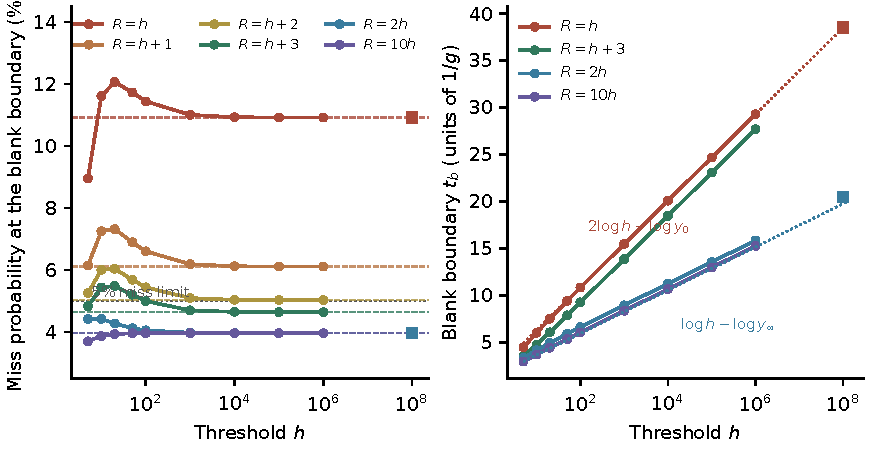
\includegraphics[width=\linewidth]{large_threshold.pdf}
\caption{Left: miss probability at the blank boundary as a function of the threshold $h$ for fixed headroom $R=h,\dots,h+3$ and fixed ratio $R=2h,10h$ (numerical, Laplace inversion; squares at $h=10^{8}$); dashed lines are the limits of Table~\ref{tab:limits}. Right: the blank boundary itself grows like $\log h$ in the reserve regime and like $2\log h$ at saturation.}\label{fig:large}
\end{figure}

\begin{figure}[htbp]\centering
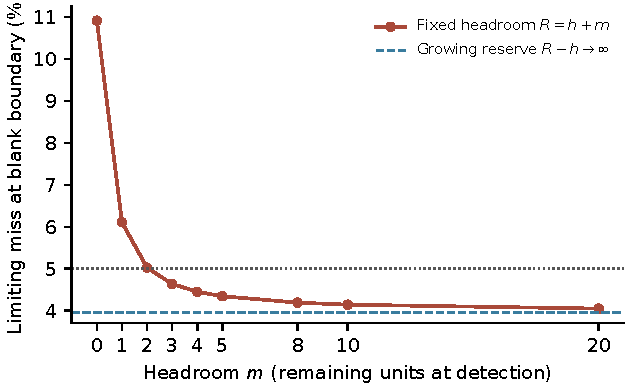
\includegraphics[width=.62\linewidth]{headroom_limit.pdf}
\caption{Limiting miss at the blank boundary as a function of the headroom $m$ (numerical). With these parameters at most two remaining units leave no window in the limit; the reserve limit is the undepleted value.}\label{fig:headroom}
\end{figure}

\subsection{What the large-threshold behaviour means for diagnostic detection}\label{sec:meaning}
\begin{enumerate}[label=(\arabic*)]
\item \emph{The effect is not a small-count artefact.} Its cause is the order-one holding time of the last few births before resource exhaustion, which is independent of $h$; Theorem~\ref{thm:big} exhibits it at $h=10^{8}$, where the fraction of reactions positive at time zero is negligible and the Poisson loading is a vanishing fraction of the threshold.
\item \emph{Absolute headroom, not the capacity ratio, decides.} A capacity that exceeds the detection threshold by a growing margin restores the undepleted design rules after a common delay $d_h$; a capacity that exceeds it by a fixed number of units does not, and the limiting tradeoff is then a function of $(b/g,\lambda,m)$. For a real assay the question becomes measurable: how many effective units remain when the detector fires. Increasing $h$ alone cannot answer it.
\item \emph{Deadlines grow logarithmically, windows do not shrink.} In units of $1/g$ the blank boundary is $\log h+d_h-\log y$ in the reserve regime and $2\log h-\log y_m$ at fixed headroom (Figure~\ref{fig:large}, right); at $h=10^{8}$ and $g=1$ per minute these are about $20$ and $38$ minutes. The width of a nonempty window converges to a positive limit, so the timing tolerance available to the instrument does not deteriorate with threshold, and an observation grid of a few seconds is not the obstruction at large $h$ that it is at $h=5$. In the fixed-rate-constant family of Proposition~\ref{prop:massaction} the time unit is $V/(k_gR)$, so physical deadlines and widths scale like $(\log R)/R$ and $1/R$; whether a real assay follows that family is part of the open calibration question.
\item \emph{The reserve limit is strictly feasible; saturation is not.} With $a=0.01$ and $\lambda=4$ the undepleted limit has miss $3.96\%$ at the blank boundary, so any assay design that keeps a growing reserve will have a window at large thresholds. A design that consumes essentially all of its effective resource at detection will not, whatever the threshold, and no re-timing repairs it.
\item \emph{The universal tradeoff is a benchmark.} Since the limit laws are explicit gamma and product-gamma laws, inference or optimisation software for stochastic assay design can be tested against them without any molecular calibration.
\end{enumerate}

\section{Data boundary, a discriminating experiment and sampling confidence}\label{sec:data}

\paragraph{Public example.} The saved digital-NAAT example distributed with the Ismagilov laboratory's melt-curve analyser \citep{ismagilovcode} contains $258$ wells and $185$ amplification frames. Reapplying its strict crossing rule (baseline-corrected intensity greater than $250$) reproduces all $29$ saved crossings with no mismatch; the other $229$ wells are retained as right-censored non-crossers, giving an all-well detection fraction $29/258\approx0.1124$ rather than the positive-only distribution that ends at one. This is a replay of the observation rule, not a fit or validation of the source: the example has no verified matched blank/loading labels, resource levels or independent run identifiers, and the unobserved future of the non-crossers is not identified by the recorded frames. Three candidate dilution and formulation workbooks in a related deposit \citep{jue2019data} returned HTTP 403 during this investigation; their controls remain unassessed, which does not establish that they are unsuitable. Melt information is available only after amplification and cannot be used by a rule that must decide earlier.

\paragraph{A discriminating experiment.} The prediction that separates the finite-resource source from a common clock change is a change in the sensitivity--blank tradeoff under a controlled resource intervention, not merely a shift of all crossing times. A study should retain matched blanks and known loading, all trajectories including non-crossers, and independent run labels across at least two measured resource conditions; fit a declared subset, freeze the source and decision rule, and test a withheld condition against an empirical crossing-time model with common acceleration. Section~\ref{sec:meaning} adds a second, sharper prediction: the effect should depend on the headroom at detection and disappear when the reserve is large. Outcomes that would change the model include a pure common-clock shift, unequal target and background growth, delayed activation or extinction in the low-loading tail, and readout noise or run heterogeneity larger than the tolerance of Theorem~\ref{thm:robust}.

\paragraph{Sampling confidence is separate from operating probability.} For a prespecified deadline and independent identically distributed reactions, zero errors in $n$ trials give the exact one-sided upper confidence bound $1-\delta^{1/n}$ at level $1-\delta$ \citep{clopperpearson1934,hanley1983}. Allocating $\delta=0.025$ to each error limit, $0.99^{368}\le0.025$ and $0.95^{72}\le0.025$, so zero errors in $368$ blanks and $72$ positive reactions give simultaneous one-sided confidence bounds at total level $95\%$ by the union bound. This planning calculation covers neither unmodelled batch variation nor selection of the deadline from the same observations, and the $1\%$ and $5\%$ model limits and the $95\%$ statistical confidence must not share an unlabelled axis. An OR rule across $m$ independent blank reactions has false-positive probability $1-(1-\alpha)^m$, not $\alpha$; the paper makes no specimen-level claim.

\section{Verification and reproducibility}\label{sec:verification}

\paragraph{Lean-verified.} The following are theorems of the frozen Lean~4 project (toolchain \lean{leanprover/lean4:v4.30.0}, pinned Mathlib manifest with SHA-256 prefix \texttt{a8df0b60}), compiled with warnings treated as errors and with their declaration interfaces authenticated; each depends only on the axioms \lean{propext}, \lean{Classical.choice} and \lean{Quot.sound}. No admitted proof, extra probability axiom or native computation is involved. The reusable probability layer is \lean{FiniteCopy/FiniteKernel} and \lean{FiniteCopy/PoissonKernel}; the development is in \lean{proofs/DiagnosticWindows}.
\begin{itemize}
\item The normalized six-state source \eqref{eq:kernel}, its nonnegativity and row sums, the latch indicator and the fact that supported moves increase the count by at most one (\lean{birthKernel}, \lean{birth_aggregates}); the literal rate formula \eqref{eq:rates} at each capacity (\lean{capacityR_rates}).
\item The infinite loading mixture \eqref{eq:miss} and its exact finite reduction (\lean{loadedSurvival}, \lean{loading_finite}); the empty-loading floor \eqref{eq:floor} (\lean{empty_loading_floor}).
\item The spectral identities and exact five-exponential survival formulas for capacities five to ten (\lean{spectral_survival}, \lean{capacityR_survival}); time monotonicity from dissipation (\lean{spectral_antitone}).
\item The exponential enclosure scheme (\lean{exp_enclosure16}) and its $11+51$ rational certificates; the certified inequalities of Table~\ref{tab:certs} and of Theorem~\ref{thm:robust}.
\item Theorem~\ref{thm:capacity}: \lean{minimum_capacity_certificates} (parts (a), (b)) and \lean{capacity10_interval} (part (c)); the original two-capacity contrast \lean{main}.
\item Rate order, loading order and the scaling identity (\lean{birth_survival_order}, \lean{loading_antitone}, \lean{scaled_survival}), and the existence equivalence of Proposition~\ref{prop:clock} (\lean{clock_feasibility_iff}).
\item Theorem~\ref{thm:robust}: \lean{robust_guarantee}.
\end{itemize}
The strict receipts for \lean{Windows.lean} (\lean{minimum_capacity_certificates}; source SHA-256 prefix \texttt{08b9fdef}, 14 dependency modules, 31 s), \lean{Robustness.lean} (\lean{robust_guarantee}; \texttt{67d6b291}, 18 modules, 79 s) and \lean{Main.lean} (\lean{main}; \texttt{493d2290}, 103 s) accompany the sources. Appendix~\ref{app:map} maps each claim to its declaration.

\paragraph{Conventional.} Lemmas~\ref{lem:separating} and \ref{lem:interval} as stated for general $R$ (their instances are Lean-verified); Proposition~\ref{prop:massaction}; all of Section~\ref{sec:large} and Appendices~\ref{app:big}--\ref{app:arith}. A Lean development of Section~\ref{sec:large} would have to formalize the identification of the uniformized law with independent holding times, the beta law and beta--gamma coupling, the variance bounds, and the four enclosures; the last are within reach of the existing enclosure scheme, the first three are not yet formalized.

\paragraph{Numerical.} The decimal displays in every table; the window endpoints and $\lambda_{\min}$ values; the undepleted reference at $2.8$ minutes; the mass-action grid witness; Table~\ref{tab:limits}, Table~\ref{tab:big} and Figures~\ref{fig:large}--\ref{fig:headroom}; the earlier threshold-twenty check (capacity $20$ at $8.0$ minutes: blank $.01341831$, miss $.08764661$; capacity $40$ at $4.8$: $.00908692$, $.04637034$), now superseded as a stress test by Theorem~\ref{thm:big} but retained as a data point in Figure~\ref{fig:large}.

\paragraph{Reproducibility.} The paper source directory contains \path{check_paper.py}, which recomputes the rational eigenvector decompositions, evaluates every witness of Table~\ref{tab:certs} in 40-digit arithmetic, replays the directed-rounding enclosures of Appendix~\ref{app:arith} and reports 41 checks; \path{large_threshold.py}, which performs the Laplace inversion and the limit-law quadratures; and \path{make_figures.py}. The problem workspace of the repository retains the certificate generators, the strict receipts with dependency manifests, the public-example replay with download hashes, and the original figure scripts. \RepositoryNote

\section{Conclusion and open problems}\label{sec:conclusion}
For an explicit finite-resource amplification source, exact certificates settle whether a usable readout deadline exists, what a prescribed observation grid does to that answer, and how much fixed-rate, loading and timing uncertainty a feasible design tolerates; these are Lean-verified at threshold five. A common clock change cannot create a window; a state-dependent resource change can. At large thresholds the holding-time representation reduces the question to explicit gamma and product-gamma laws: a growing reserve restores the undepleted rules after a deterministic delay, a fixed headroom does not, and for every $h\ge10^{8}$ the contrast between saturation and a doubled capacity is proved with explicit constants.

Open problems. (1) A measured interpretation of effective capacity, background and growth in a real assay, and a test of the headroom prediction under a controlled resource intervention. (2) A quantitative finite-threshold classification of the minimal headroom, which the numerical results suggest is three at $h=5$ and in the limit but four at intermediate thresholds. (3) Formalization of the holding-time and beta--gamma arguments, which would bring Section~\ref{sec:large} to the same evidence level as Section~\ref{sec:certified}. (4) Extensions with activation delay, loss, unequal target and background growth, readout noise, time-dependent rates or adaptive stopping, each of which changes the source and needs its own analysis. (5) Specimen-level rules that aggregate several reactions.

\appendix

\section{Exact source calculation and rational enclosures}\label{app:exact}
Write $r_z=q_R(z)/\nu$ and $P=P_R$. For each of the six capacities the five transient rates are distinct, and the uncalled indicator is a sum of five eigenvectors,
\[
f=\sum_{i=0}^{4}V_i,\qquad PV_i=e_iV_i,\qquad e_i=1-r_i.
\]
To construct $V_i$, set its entries above $i$ (including at the absorbing state) to zero and use the backward recurrence
\begin{equation}\label{eq:recurrence}
V_i(z)=\frac{q_R(z)}{q_R(z)-q_R(i)}\,V_i(z+1)\qquad(z<i),
\end{equation}
choosing $V_i(i)$ from $i=4$ down to $0$ so that $\sum_jV_j(i)=1$. Every coefficient is rational; Lean checks the decomposition and each eigenvector equation against the literal kernel by direct substitution. Induction gives $P^nV_i=e_i^nV_i$, and summing the Poisson series in \eqref{eq:source} yields
\begin{equation}\label{eq:spectral}
S_R(t,z)=\sum_{i=0}^{4}e^{-q_R(i)t}\,V_i(z).
\end{equation}
The components may have signed entries; positivity is a property of the kernel, not of this representation. Near-coincident rates produce large cancelling coefficients: at capacity five, where $q_5(2)=1.206$ and $q_5(3)=1.204$, the loaded coefficients exceed $4900$ in absolute value (over $11{,}000$ at capacity seven). Floating-point agreement was therefore not accepted as a certificate.

\begin{lemma}[Time monotonicity; Lean-verified]\label{lem:antitone}
$S_R(t,z)$ is nonincreasing in $t\ge0$ for every $z$.
\end{lemma}
\begin{proof}
$Pf\le f$ because $f$ is nonincreasing on the states and $P$ moves upward. In the uniformization clock $u=\nu t$ put $d=Pf-f=\sum_i(e_i-1)V_i\le0$. Differentiating \eqref{eq:spectral},
\[
\frac{\dd}{\dd u}\sum_ie^{u(e_i-1)}V_i(z)=\sum_ie^{u(e_i-1)}(e_i-1)V_i(z)=\sum_{n\ge0}e^{-u}\frac{u^n}{n!}(P^nd)(z)\le0,
\]
the last inequality by kernel positivity. Nonnegative Poisson loading weights preserve the order.
\end{proof}

\paragraph{Rational enclosures.} At a rational deadline every exponent in \eqref{eq:spectral} is rational. For each required exponent $x$ let $y=x/16$, so $|y|\le1$, and put $A(y)=\sum_{j=0}^{11}y^j/j!$ and $B(y)=13|y|^{12}/(12\cdot12!)$. The Taylor remainder bound available in Mathlib gives $A(y)-B(y)\le e^y\le A(y)+B(y)$. Rational $l,u$ are chosen outward at precision $10^{-12}$ with $0\le l\le A(y)-B(y)$ and $A(y)+B(y)\le u$; then $l^{16}\le e^x\le u^{16}$, and a final outward rounding at $10^{-9}$ gives compact endpoints. Each step, including the sign-sensitive propagation of the enclosures through \eqref{eq:spectral} and \eqref{eq:miss}, is checked in Lean. The robustness endpoints use loading $4$ for the blank bound and the exact mean $399/100$ for the miss bound; no displayed decimal is a premise.

\section{Comparison lemmas for the source law}\label{app:comparisons}
Let $P_r$ be a pure-birth kernel on $\{0,\dots,5\}$ with jump probabilities $0\le r_z\le1$ and absorbing state five.

\begin{lemma}[Rate order; Lean-verified]\label{lem:rateorder}
If $a$ is nonincreasing on the states then so is $P_ra$. If $r_z\le s_z$ for all $z$ then $P_s^nf\le P_r^nf$ for all $n$, hence $S_s(t,z)\le S_r(t,z)$ and, after loading, $M_{s,\lambda}\le M_{r,\lambda}$. Also $S_r(t,z)$ is nonincreasing in $z$.
\end{lemma}
\begin{proof}
$(P_ra)(z)=(1-r_z)a(z)+r_za(z+1)$ lies between $a(z+1)$ and $a(z)$; for $x<y$, $(P_ra)(x)\ge a(x+1)\ge a(y)\ge(P_ra)(y)$. No increasing-rate assumption is needed. If $r_z\le s_z$ then $(P_sa)(z)-(P_ra)(z)=(s_z-r_z)(a(z+1)-a(z))\le0$; positivity and induction give the order for powers, and nonnegative Poisson weights give it for \eqref{eq:source} and \eqref{eq:miss}.
\end{proof}

\begin{lemma}[Loading order; Lean-verified]\label{lem:loadorder}
For fixed $t$, $\lambda\mapsto M_{R,\lambda}(t)$ is nonincreasing on $[0,\infty)$.
\end{lemma}
\begin{proof}
With $a_n=S(t,n)$, $a_5=0$, nonnegative and nonincreasing,
\[
\frac{\dd}{\dd\lambda}\Bigl[e^{-\lambda}\sum_{n=0}^{4}\frac{\lambda^n}{n!}a_n\Bigr]
=e^{-\lambda}\Bigl[\sum_{n=0}^{3}\frac{\lambda^n}{n!}(a_{n+1}-a_n)-\frac{\lambda^4}{24}a_4\Bigr]\le0.\qedhere
\]
\end{proof}

\begin{lemma}[Rate scaling; Lean-verified]\label{lem:scaling}
If $cr_z\le1$ for all $z$ then $P_{cr}=cP_r+(1-c)I$, its action on an eigenvector of eigenvalue $e_i$ is multiplication by $1+c(e_i-1)$, and $S_{cr}(u,z)=S_r(cu,z)$; the same identity holds after loading. For arbitrary $c>0$, uniformizing the rates $cq_z$ at $c\nu$ leaves the normalized kernel unchanged and scales its Poisson clock, which gives Proposition~\ref{prop:clock}.
\end{lemma}

\section{Proof of Theorem~\ref{thm:big}}\label{app:big}
Fix $a=1/100$, $\eps=1/100$, $n_*=25$ and $C=10{,}000+(20{,}000/199)^2$. All times are in units of $1/g$.

\paragraph{Concentration inequalities.} For $Z\sim\Gam(s,1)$, the event $|\log(Z/s)|>\eps$ implies $|Z-s|>s(1-e^{-\eps})$, so by Chebyshev
\begin{equation}\label{eq:gammacheb}
\Prob\bigl(|\log(Z/s)|>\eps\bigr)\le\frac{1}{s(1-e^{-\eps})^2}\le\frac{(20{,}000/199)^2}{s},
\end{equation}
using $1-e^{-\eps}\ge\eps-\eps^2/2=199/20{,}000$. For $h\ge10^{8}$ put
\begin{equation}\label{eq:deltas}
\delta_+=C/h<0.000202,\qquad\delta_-=(401/100)\,C/h<0.000807,
\end{equation}
and note $\Prob(N>25)\le e^{-4}\frac{4^{26}}{26!}\bigl(1-\frac4{27}\bigr)^{-1}<3\times10^{-13}$ and $25/(h-24)<3\times10^{-7}$.

\paragraph{Elementary bounds on the limit laws.} (i) $99\le\Gamma(a)\le100$: with $X\sim\Ex(1)$, $\Gamma(a)=\E[X^a]/a$, concavity gives $\E X^a\le1$, and $X^a\ge1+a\log X$ with $\E\log X=-\gamma\ge-1$ gives $\E X^a\ge1-a$. (ii) From $w^a\le1-a+aw$,
\begin{equation}\label{eq:blankup}
\Prob(\Gam(a,1)\ge y)\le0.01\,E_1(y)+\frac{0.01}{99}e^{-y},\qquad E_1(y)=\int_y^\infty\frac{e^{-w}}{w}\dd w.
\end{equation}
(iii) For $n\ge1$, $\Gam(n+a)$ stochastically dominates $\Gam(n)$ and $\Prob(\Gam(n,1)\le y)\le y^n/n!$; bounding the $n=0$ term by one,
\begin{equation}\label{eq:missup}
\sum_{n\ge0}\Prob(N=n)\Prob(\Gam(n+a,1)\le y)\le e^{-4}\sum_{n\ge0}\frac{(4y)^n}{(n!)^2}=e^{-4}I_0(4\sqrt y).
\end{equation}
(iv) For $Y\sim\Ex(1)$ independent of $W\sim\Gam(a,1)$, since $0.97^{100}<0.05$ gives $w^a\ge0.97$ on $w\ge0.05$,
\begin{equation}\label{eq:blanklow}
\Prob(WY\ge y)=\frac1{\Gamma(a)}\int_0^\infty w^{a-1}e^{-w-y/w}\dd w\ge0.0097\int_{0.05}^{10}\frac{e^{-w-y/w}}{w}\dd w.
\end{equation}
(v) For $W_n\sim\Gam(n+a,1)$, by $1-e^{-u}\ge u/(1+u)$ and the convexity of $w\mapsto y/(w+y)$,
\begin{equation}\label{eq:misslow}
\Prob(W_nY\le y)=\E\bigl[1-e^{-y/W_n}\bigr]\ge\E\Bigl[\frac{y}{W_n+y}\Bigr]\ge\frac{y}{n+a+y}.
\end{equation}

\paragraph{(a) Capacity $2h$.} By Lemma~\ref{lem:holding}, $T_{2h,h,n}=A_{h,n}+D_n$ with $D_n=\sum_{z=n}^{h-1}\frac{zE_z}{(z+a)(2h-z)}$, $\Var D_n\le\sum_{z<h}(2h-z)^{-2}\le1/h$, and $|\E D_n-\mu_+(h)|\le25/(h-24)$ for $n\le25$. By Lemma~\ref{lem:beta}, $A_{h,n}=\log Z-\log W_n$ with $Z\sim\Gam(h+a,1)$, $W_n\sim\Gam(n+a,1)$. Apply Chebyshev to $D_n$ (probability at most $\Var D_n/\eps^2\le10^4/h$) and \eqref{eq:gammacheb} to $Z$; outside an event of probability at most $\delta_+$,
\begin{equation}\label{eq:goodplus}
\bigl|T_{2h,h,n}-\log(h+a)-\mu_+(h)+\log W_n\bigr|\le2\eps+\frac{25}{h-24}<0.020001.
\end{equation}
At $t_+$ of \eqref{eq:tplus}, on the good event, $T_{2h,h,0}\le t_+$ forces $W_0\ge0.3e^{-0.020001}>0.293$, and $T_{2h,h,n}>t_+$ forces $W_n<0.3e^{0.020001}<0.307$. Hence
\begin{align*}
F_{0,2h}(t_+)&\le\Prob(\Gam(a,1)\ge0.293)+\delta_+,\\
M_{2h,4}(t_+)&\le\sum_{n\ge0}\Prob(N=n)\Prob(\Gam(n+a,1)\le0.307)+\delta_++3\times10^{-13},
\end{align*}
where loads $n>25$ are covered by the Poisson tail and loads $n\ge h$ are absorbed. By \eqref{eq:blankup}, \eqref{eq:missup} and the enclosures of Appendix~\ref{app:arith},
\[
0.01E_1(0.293)+\tfrac{0.01}{99}e^{-0.293}<0.009372,\qquad e^{-4}\sum_{n\ge0}\frac{1.228^n}{(n!)^2}<0.048731,
\]
so $F_{0,2h}(t_+)<0.009372+0.000202<0.00958$ and $M_{2h,4}(t_+)<0.048731+0.000202+3\times10^{-13}<0.04894$.

\paragraph{(b) Capacity $h$.} With $c_h=h/(h+a)$, $k=\lfloor h/2\rfloor$, $\ell=h-k$, Lemma~\ref{lem:holding} gives $T_{h,h,n}/c_h=U_n+V+C_n$ as in the proof of Theorem~\ref{thm:headroom}, with $e^{-U_n}\sim\Bet(n+a,k-n)$ and $e^{-V}\sim\Bet(1,\ell)$ independent. Apply the coupling of Lemma~\ref{lem:beta} to each block: $U_n=\log Z_1-\log W_n$ and $V=\log Z_2-\log Y$ with $Z_1\sim\Gam(k+a,1)$, $Z_2\sim\Gam(\ell+1,1)$, $W_n\sim\Gam(n+a,1)$, $Y\sim\Ex(1)$, and $W_n$, $Y$ independent. Every coefficient in $C_n$ is at most $1/k$ and there are at most $h$ of them, so $\Var C_n\le h/k^2\le4h/(h-1)^2\le4.01/h$; likewise $1/(k+a)+1/(\ell+1)\le2/k\le4.01/h$; and $|\E C_n-\mu_-(h)|\le25/(h-24)$ for $n\le25$. Chebyshev on $C_n$ and \eqref{eq:gammacheb} on $Z_1,Z_2$ give, outside an event of probability at most $\delta_-$,
\begin{equation}\label{eq:goodminus}
\bigl|T_{h,h,n}/c_h-\log(k+a)-\log(\ell+1)-\mu_-(h)+\log(W_nY)\bigr|<0.030001.
\end{equation}
At $t_-$ of \eqref{eq:tminus}, on the good event, $W_0Y\ge0.155>0.15e^{0.030001}$ forces $T_{h,h,0}\le t_-$, and $W_nY\le0.145<0.15e^{-0.030001}$ forces $T_{h,h,n}>t_-$. Hence
\begin{align*}
F_{0,h}(t_-)&\ge\Prob(\Gam(a,1)\,Y\ge0.155)-\delta_-,\\
M_{h,4}(t_-)&\ge e^{-4}\sum_{n=0}^{5}\frac{4^n}{n!}\,\frac{0.145}{n+0.155}-\delta_-,
\end{align*}
using \eqref{eq:misslow} and keeping only the nonnegative loads $n\le5$. By \eqref{eq:blanklow} and Appendix~\ref{app:arith}, $\Prob(\Gam(a,1)Y\ge0.155)>0.01087$ and the finite sum exceeds $0.056383$, so $F_{0,h}(t_-)>0.01087-0.000807>0.01006$ and $M_{h,4}(t_-)>0.056383-0.000807>0.0555$. Both limits are strictly violated at $t_-$, and Lemma~\ref{lem:separating} excludes every deadline. \qed

\section{Directed arithmetic for the four enclosures}\label{app:arith}
The four scalar bounds used in Appendix~\ref{app:big} are evaluated in \path{check_paper.py} with Python's \texttt{decimal} module at 50 digits and explicit rounding directions, so that each printed bound is an outward bound of the corresponding exact quantity. For $0\le u\le1$ the Taylor polynomial of degree eleven lies below $e^u$ and adding $13u^{12}/(12\cdot12!)$ gives an upper bound; scaling by $32$ and squaring five times encloses $e^{x}$ for $0\le x\le32$, and reciprocation encloses $e^{-x}$. The exponential integral is bounded above by an upper Riemann sum on $[0.293,20]$ with step $0.005$ plus the tail $e^{-20}/20$; the series $\sum1.228^n/(n!)^2$ is summed to $n=20$ with a geometric tail; the Poisson tail uses its first omitted term and a geometric ratio $4/27$; the integral in \eqref{eq:blanklow} is bounded below by a lower Riemann sum on $[0.05,10]$ with step $0.005$, using the convexity of $w+0.155/w$ on each subinterval. The results are
\begin{center}\small
\begin{tabular}{lr}\toprule
Quantity & Directed bound\\\midrule
capacity $2h$, blank upper bound, after adding $\delta_+$ & $0.0095725$\\
capacity $2h$, miss upper bound, after adding $\delta_+$ and the Poisson tail & $0.0489313$\\
capacity $h$, blank lower bound, after subtracting $\delta_-$ & $0.0100703$\\
capacity $h$, miss lower bound, after subtracting $\delta_-$ & $0.0555773$\\\bottomrule
\end{tabular}
\end{center}
and the script asserts the coarser inequalities $<0.00958$, $<0.04894$, $>0.01006$, $>0.0555$ used in the theorem. An independent evaluation with \texttt{mpmath} at 40 digits agrees with each bound to the printed digits; the exact limiting quantities are more favourable still ($\Prob(\Gam(a)\ge0.293)=0.009247$, $\Prob(\Gam(a)Y\ge0.155)=0.011485$). The arithmetic is $h$-independent except through the allowances $\delta_\pm$, which decrease with $h$.

\section{Claims-to-declarations map}\label{app:map}
\begin{center}\small
\begin{tabular}{>{\raggedright\arraybackslash}p{.36\linewidth}>{\raggedright\arraybackslash}p{.58\linewidth}}\toprule
Claim & Lean declaration(s) in namespace \texttt{DiagnosticWindows}\\\midrule
Source kernel, positivity, row sums, latch & \lean{birthKernel}, \lean{uncalled_indicator}, \lean{birth_aggregates} (BirthSource)\\
Loading mixture, exact finite reduction, floor \eqref{eq:floor} & \lean{loadedSurvival}, \lean{loading_finite}, \lean{empty_loading_floor} (Loading)\\
Spectral survival, monotonicity from dissipation & \lean{spectral_survival} (Spectral), \lean{spectral_antitone} (Monotonicity)\\
Rational eigenvectors, rates, survival formulas $R=5,\dots,10$ & \lean{capacityR_rates}, \lean{capacityR_sum}, \lean{capacityR_eigen}, \lean{capacityR_survival} (Capacity, ExtraCapacity)\\
Exponential enclosures & \lean{exp_enclosure16} (ExponentialBounds); 11 certificates (ExpCertificates); 51 certificates \lean{post_exp_i} (WindowCertificates)\\
Table~\ref{tab:certs} inequalities & \lean{capacity5_separating_errors}, \lean{capacity10_errors} (Numerical); \lean{rR_blank_bound}, \lean{rR_miss_bound}, \lean{r8early_miss_bound}, \lean{r8late_blank_bound}, \lean{interval_early_miss_bound}, \lean{interval_late_blank_bound} (WindowCertificates)\\
Theorem~\ref{thm:capacity}(a),(b) & \lean{capacityR_no_deadline}, \lean{capacity8_grid_impossible}, \lean{minimum_capacity_certificates} (Windows)\\
Theorem~\ref{thm:capacity}(c) & \lean{capacity10_interval} (Windows)\\
Original two-capacity contrast & \lean{main} (Main)\\
Lemma~\ref{lem:rateorder} & \lean{birth_step_antitone}, \lean{birth_survival_order}, \lean{birth_survival_antitone_state} (Comparison)\\
Lemma~\ref{lem:loadorder} & \lean{loading_antitone}, \lean{loaded_rate_order} (LoadingOrder)\\
Lemma~\ref{lem:scaling}, Proposition~\ref{prop:clock} & \lean{scaled_survival}, \lean{scaled10_loading}, \lean{clock_feasibility_iff} (RateScale)\\
Theorem~\ref{thm:robust} & \lean{robust_blank_blank_bound}, \lean{robust_miss_miss_bound} (WindowCertificates); \lean{robust_guarantee} (Robustness)\\\bottomrule
\end{tabular}
\end{center}

\bibliographystyle{plainnat}
\small
\bibliography{refs}

\end{document}
